\documentclass{standalone}
\usepackage{tikz}
\usetikzlibrary{patterns, positioning}


\begin{document}
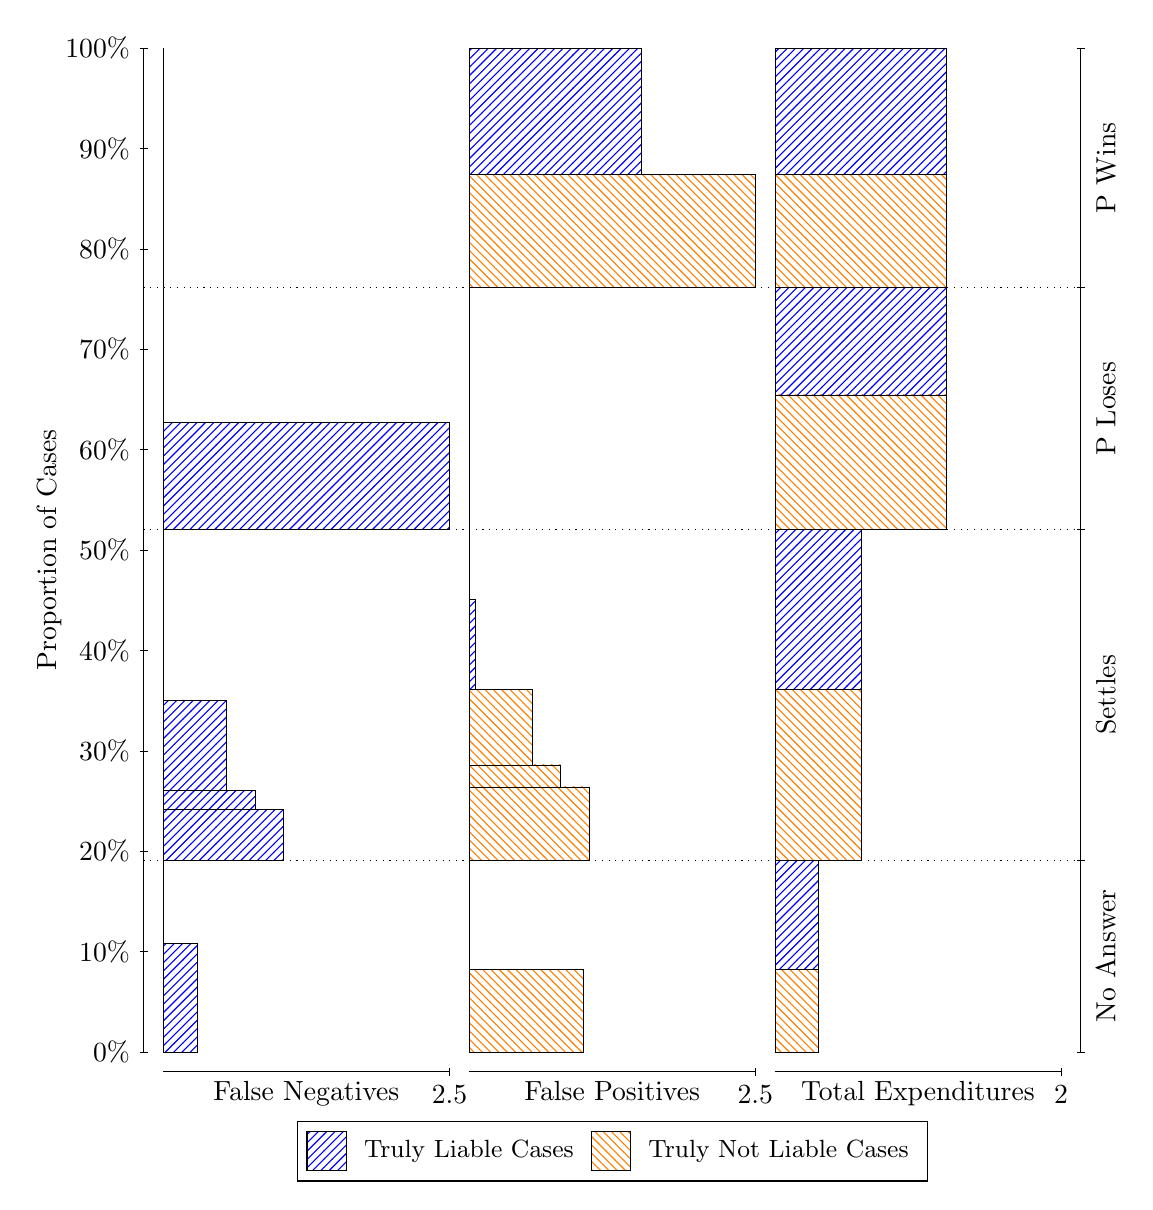
\begin{tikzpicture}
\draw[black, very thin] (1.5,1.75) -- (1.5,14.5);
\node[rotate=90, text=black, anchor=center] at (0.3, 8.125) {Proportion of Cases};
\draw[black, very thin] (1.45,1.75) -- (1.55,1.75);
\node[text=black, anchor=east] at (1.45, 1.75) {0\%};
\draw[black, very thin] (1.45,3.025) -- (1.55,3.025);
\node[text=black, anchor=east] at (1.45, 3.025) {10\%};
\draw[black, very thin] (1.45,4.3) -- (1.55,4.3);
\node[text=black, anchor=east] at (1.45, 4.3) {20\%};
\draw[black, very thin] (1.45,5.575) -- (1.55,5.575);
\node[text=black, anchor=east] at (1.45, 5.575) {30\%};
\draw[black, very thin] (1.45,6.85) -- (1.55,6.85);
\node[text=black, anchor=east] at (1.45, 6.85) {40\%};
\draw[black, very thin] (1.45,8.125) -- (1.55,8.125);
\node[text=black, anchor=east] at (1.45, 8.125) {50\%};
\draw[black, very thin] (1.45,9.4) -- (1.55,9.4);
\node[text=black, anchor=east] at (1.45, 9.4) {60\%};
\draw[black, very thin] (1.45,10.675) -- (1.55,10.675);
\node[text=black, anchor=east] at (1.45, 10.675) {70\%};
\draw[black, very thin] (1.45,11.95) -- (1.55,11.95);
\node[text=black, anchor=east] at (1.45, 11.95) {80\%};
\draw[black, very thin] (1.45,13.225) -- (1.55,13.225);
\node[text=black, anchor=east] at (1.45, 13.225) {90\%};
\draw[black, very thin] (1.45,14.5) -- (1.55,14.5);
\node[text=black, anchor=east] at (1.45, 14.5) {100\%};

\draw[black, very thin] (13.4,1.75) -- (13.4,14.5);
\draw[black, very thin] (13.35,1.75) -- (13.45,1.75);
\node[anchor=west] at (13.35, 1.75) {};
\draw[black, very thin] (13.35,4.1861) -- (13.45,4.1861);
\node[anchor=west] at (13.35, 4.1861) {};
\draw[black, very thin] (13.35,8.3834) -- (13.45,8.3834);
\node[anchor=west] at (13.35, 8.3834) {};
\draw[black, very thin] (13.35,11.457) -- (13.45,11.457);
\node[anchor=west] at (13.35, 11.457) {};
\draw[black, very thin] (13.35,14.5) -- (13.45,14.5);
\node[anchor=west] at (13.35, 14.5) {};

\draw[black, very thin, pattern color=blue, pattern=north east lines] (1.75,1.75) rectangle (2.186,3.1338);
\draw[black, very thin, pattern color=orange, pattern=north west lines] (1.75,3.1338) rectangle (1.75,4.1861);
\draw[black, very thin, pattern color=blue, pattern=north east lines] (1.75,4.1861) rectangle (3.276,4.8303);
\draw[black, very thin, pattern color=blue, pattern=north east lines] (1.75,4.8303) rectangle (2.9127,5.0741);
\draw[black, very thin, pattern color=blue, pattern=north east lines] (1.75,5.0741) rectangle (2.5493,6.2168);
\draw[black, very thin, pattern color=orange, pattern=north west lines] (1.75,6.2168) rectangle (1.75,8.3834);
\draw[black, very thin, pattern color=blue, pattern=north east lines] (1.75,8.3834) rectangle (5.3833,9.744);
\draw[black, very thin, pattern color=orange, pattern=north west lines] (1.75,9.744) rectangle (1.75,11.457);
\draw[black, very thin, pattern color=orange, pattern=north west lines] (1.75,11.457) rectangle (1.75,12.9);
\draw[black, very thin, pattern color=blue, pattern=north east lines] (1.75,12.9) rectangle (1.75,14.5);
\draw[black, very thin, pattern color=orange, pattern=north west lines] (5.6333,1.75) rectangle (7.0867,2.8023);
\draw[black, very thin, pattern color=blue, pattern=north east lines] (5.6333,2.8023) rectangle (5.6333,4.1861);
\draw[black, very thin, pattern color=orange, pattern=north west lines] (5.6333,4.1861) rectangle (7.1593,5.1173);
\draw[black, very thin, pattern color=orange, pattern=north west lines] (5.6333,5.1173) rectangle (6.796,5.3948);
\draw[black, very thin, pattern color=orange, pattern=north west lines] (5.6333,5.3948) rectangle (6.4327,6.3527);
\draw[black, very thin, pattern color=blue, pattern=north east lines] (5.6333,6.3527) rectangle (5.706,7.4955);
\draw[black, very thin, pattern color=blue, pattern=north east lines] (5.6333,7.4955) rectangle (5.6333,8.3834);
\draw[black, very thin, pattern color=orange, pattern=north west lines] (5.6333,8.3834) rectangle (5.6333,10.096);
\draw[black, very thin, pattern color=blue, pattern=north east lines] (5.6333,10.096) rectangle (5.6333,11.457);
\draw[black, very thin, pattern color=orange, pattern=north west lines] (5.6333,11.457) rectangle (9.2667,12.9);
\draw[black, very thin, pattern color=blue, pattern=north east lines] (5.6333,12.9) rectangle (7.8133,14.5);
\draw[black, very thin, pattern color=orange, pattern=north west lines] (9.5167,1.75) rectangle (10.062,2.8023);
\draw[black, very thin, pattern color=blue, pattern=north east lines] (9.5167,2.8023) rectangle (10.062,4.1861);
\draw[black, very thin, pattern color=orange, pattern=north west lines] (9.5167,4.1861) rectangle (10.607,6.3527);
\draw[black, very thin, pattern color=blue, pattern=north east lines] (9.5167,6.3527) rectangle (10.607,8.3834);
\draw[black, very thin, pattern color=orange, pattern=north west lines] (9.5167,8.3834) rectangle (11.697,10.096);
\draw[black, very thin, pattern color=blue, pattern=north east lines] (9.5167,10.096) rectangle (11.697,11.457);
\draw[black, very thin, pattern color=orange, pattern=north west lines] (9.5167,11.457) rectangle (11.697,12.9);
\draw[black, very thin, pattern color=blue, pattern=north east lines] (9.5167,12.9) rectangle (11.697,14.5);
\draw[black, dotted] (1.5,4.1861) -- (13.4,4.1861);
\draw[black, dotted] (1.5,8.3834) -- (13.4,8.3834);
\draw[black, dotted] (1.5,11.457) -- (13.4,11.457);
\draw[black, very thin] (1.75,1.5) -- (5.3833,1.5);
\node[text=black, anchor=north] at (3.5667, 1.5) {False Negatives};
\draw[black, very thin] (5.3833,1.45) -- (5.3833,1.55);
\node[text=black, anchor=north] at (5.3833, 1.45) {2.5};

\draw[black, very thin] (5.6333,1.5) -- (9.2667,1.5);
\node[text=black, anchor=north] at (7.45, 1.5) {False Positives};
\draw[black, very thin] (9.2667,1.45) -- (9.2667,1.55);
\node[text=black, anchor=north] at (9.2667, 1.45) {2.5};

\draw[black, very thin] (9.5167,1.5) -- (13.15,1.5);
\node[text=black, anchor=north] at (11.333, 1.5) {Total Expenditures};
\draw[black, very thin] (13.15,1.45) -- (13.15,1.55);
\node[text=black, anchor=north] at (13.15, 1.45) {2};

\node[text=black, centered, rotate=90] at (13.72, 2.9681) {No Answer};
\node[text=black, centered, rotate=90] at (13.72, 6.2848) {Settles};
\node[text=black, centered, rotate=90] at (13.72, 9.9201) {P Loses};
\node[text=black, centered, rotate=90] at (13.72, 12.978) {P Wins};

\draw (7.449999999999999,1.5) node[draw=none] (baseCoordinate) {};
\begin{scope}[align=center]
        \matrix[scale=0.5, draw=black, below=0.5cm of baseCoordinate, nodes={draw}, column sep=0.1cm]{
            \node[rectangle, draw, minimum width=0.5cm, minimum height=0.5cm, pattern color=blue, pattern=north east lines] {}; &
            \node[draw=none, font=\small, text=black] (B) {Truly Liable Cases}; &
            \node[rectangle, draw, minimum width=0.5cm, minimum height=0.5cm, pattern color=orange, pattern=north west lines] {}; &
            \node[draw=none, font=\small, text=black] (B) {Truly Not Liable Cases}; \\
            };
\end{scope}

\end{tikzpicture}
\end{document}